\documentclass[submit]{harvardml}

\course{CS181-S23}
\assignment{Assignment \#1}
\duedate{11:59pm ET, February 9, 2023} 

\usepackage[OT1]{fontenc}
\usepackage[colorlinks,citecolor=blue,urlcolor=blue]{hyperref}
\usepackage[pdftex]{graphicx}
\usepackage{graphicx}
\usepackage{caption}
\usepackage{fullpage}
\usepackage{enumitem}
\usepackage{soul}
\usepackage{amsmath}
\usepackage{amssymb}
\usepackage{color}
\usepackage{todonotes}
\usepackage{listings}
\usepackage{common}
\usepackage{framed}
\usepackage{float}

\usepackage[mmddyyyy,hhmmss]{datetime}

\definecolor{verbgray}{gray}{0.9}

\lstnewenvironment{csv}{
  \lstset{backgroundcolor=\color{verbgray},
  frame=single,
  framerule=0pt,
  basicstyle=\ttfamily,
  columns=fullflexible}}{}

 \DeclareMathOperator*{\limover}{\overline{lim}}

\begin{document}
\begin{center}
{\Large Homework 1: Regression}\\
\end{center}

\subsection*{Introduction}
This homework is on different three different forms of regression: kernelized regression, nearest neighbors regression, 
and linear regression.  We will discuss implementation and examine their tradeoffs by implementing them on the same dataset, 
which consists of temperature over the past 800,000 years taken from ice core samples.

The folder \verb|data| contains the data you will use for this problem. There are two files:
\begin{itemize}
    \item \verb|earth_temperature_sampled_train.csv| 
    \item \verb|earth_temperature_sampled_test.csv|
\end{itemize} 

Each has two columns.  The first column is the age of the ice core sample. For our purposes we can 
think of this column as the calendar year BC. The second column is the approximate difference in 
yearly temperature (K) from the mean  over a 5000 year time window starting at the given age. 
The temperatures were retrieved from ice cores in Antarctica (Jouzel 
et al. 2007)\footnote{Retrieved from \url{https://www.ncei.noaa.gov/pub/data/paleo/icecore/antarctica/epica_domec/edc3deuttemp2007.txt}


Jouzel, J., Masson-Delmotte, V., Cattani, O., Dreyfus, G., Falourd, 
S., Hoffmann, G., … Wolff, E. W. (2007). Orbital and Millennial 
Antarctic Climate Variability over the Past 800,000 Years. 
\emph{Science, 317}(5839), 793–796. doi:10.1126/science.1141038}.
 
 The following is a snippet of the data file:
 
\begin{csv}
# Age, Temperature
3.999460000000000000e+05,5.090439218398755017e+00
4.099800000000000000e+05,6.150439218398755514e+00
\end{csv}

\textbf{Due to the large magnitude of the years, we will work in terms of thousands of years BCE in Problems 1-3.} This is taken care of for you in the provided notebook.

\begin{center}
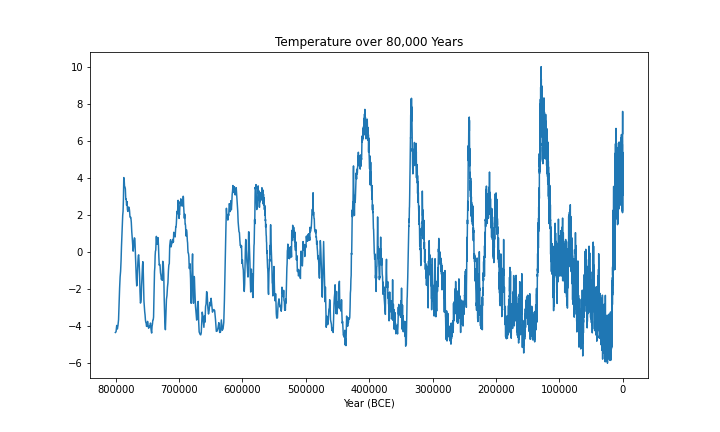
\includegraphics[width=.8\textwidth]{images/temperature}
\end{center}
\noindent 


If you find that you are having trouble with the first couple
problems, we recommend going over the fundamentals of linear algebra
and matrix calculus (see links on website).  The relevant parts of the
\href{https://github.com/harvard-ml-courses/cs181-textbook/blob/master/Textbook.pdf}{cs181-textbook notes are Sections 2.1 - 2.7}.  We strongly recommend
reading the textbook before beginning the homework.

We also encourage you to first read the \href{http://users.isr.ist.utl.pt/~wurmd/Livros/school/Bishop\%20-\%20Pattern\%20Recognition\%20And\%20Machine\%20Learning\%20-\%20Springer\%20\%202006.pdf}{Bishop textbook}, particularly:
Section 2.3 (Properties of Gaussian Distributions), Section 3.1
(Linear Basis Regression), and Section 3.3 (Bayesian Linear
Regression). (Note that our notation is slightly different but the
underlying mathematics remains the same!).

\textbf{Please type your solutions after the corresponding problems using this
\LaTeX\ template, and start each problem on a new page.} You may find
the following introductory resources on \LaTeX\ useful: 
\href{http://www.mjdenny.com/workshops/LaTeX_Intro.pdf}{\LaTeX\ Basics} 
and \href{https://www.overleaf.com/learn/latex/Free_online_introduction_to_LaTeX_(part_1)}{\LaTeX\ tutorial with exercises in Overleaf}

Homeworks will be submitted through Gradescope. You will be added to
the course Gradescope once you join the course Canvas page. If you
haven't received an invitation, contact the course staff through Ed.

\textbf{Please submit the writeup PDF to the Gradescope assignment
  `HW1'.} Remember to assign pages for each question.

\textbf{Please submit your \LaTeX file and code files to the
  Gradescope assignment `HW1 - Supplemental'.} Your files should be
named in the same way as we provide them in the repository,
e.g. \texttt{hw1.pdf}, etc.


%%%%%%%%%%%%%%%%%%%%%%%%%%%%%%%%%%%%%%%%%%%%%
% Problem 1
%%%%%%%%%%%%%%%%%%%%%%%%%%%%%%%%%%%%%%%%%%%%%
\begin{problem}[Optimizing a Kernel]
Kernel-based regression techniques are similar to nearest-neighbor
regressors: rather than fit a parametric model, they predict values
for new data points by interpolating values from existing points in
the training set.  In this problem, we will consider a kernel-based
regressor of the form:
\begin{equation*}
  f_\tau(x^*) = \cfrac{\sum_{n} K_\tau(x_n,x^*) y_n}{\sum_n K_\tau(x_n, x^*)} 
\end{equation*}
where $\{(x_n,y_n)\}_{n = 1} ^N$ are the training data points, and $K_\tau(x,x')$ is a
kernel function that defines the similarity between two inputs $x$ and
$x'$. A popular choice of kernel is a function that decays as the
distance between the two points increases, such as
\begin{equation*}
  K_\tau(x,x') = \exp\left\{-\frac{(x-x')^2}{\tau}\right\}
\end{equation*}
where $\tau$ represents the square of the lengthscale (a scalar value that 
dictates how quickly the kernel decays).  In this
problem, we will consider optimizing what that (squared) lengthscale
should be.

\noindent\emph{Make sure to include all required plots in your PDF.}

\begin{enumerate}
  
\item Let's first take a look at the behavior of the fitted model for different values of $\tau$. Plot your model for years in the range $800,000$ BC to $400,000$ BC at $1000$ year intervals for the following three values of $\tau$: $1, 50, 2500$. Since we're working in terms of thousands of years, this means you should plot $(x, f_\tau(x))$ for $x = 400, 401, \dots, 800$. The plotting has been set up for you in the notebook already.


Include your plot in your solution PDF.

\textbf{In no more than 5 sentences}, describe what happens in each of the three cases. How well do the models interpolate? If you were to choose one of these models to use for predicting the temperature at some year in this range, which would you use? 

\item Say we instead wanted to empirically evaluate which value of $\tau$ to choose. One option is to evaluate the mean squared error (MSE) for $f_{\tau}$ on the training set and simply choose the value of $\tau$ that gives the lowest loss. Why is this a bad idea?
    
Hint: consider what value of $\tau$ would be optimal, for $\tau$ ranging in $(0, \infty)$. We can consider $f_\tau(x^*)$ as a weighted average of the training responses, where the weights are proportional to the distance to $x^*$, and the distance is computed via the kernel. What happens to $K_\tau(x, x')$ as $\tau$ becomes very small, when $x = x'$? What about when $x \neq x'$?

\item We will evaluate the models by computing their MSE on the test set. 

Let $\{(x'_m, y'_m)\}_{m = 1} ^M$ denote the test set. Write down the form of the MSE of $f_\tau$ over the test set as a function of the training set and test set. Your answer may include $\{(x'_m, y'_m)\}_{m = 1} ^M$, $\{(x_n, y_n)\}_{n = 1} ^N$, and $K_\tau$, but not $f_\tau$.

\item We now compute the MSE on the provided training set. Write Python code to compute the MSE with respect to the same lengthscales as in Part 1. Which model yields the lowest test set MSE? Is this consistent with what you observed in Part 1?

\item 
Say you would like to send your friend your kernelized regressor, so that they can reproduce the same exact predictions as you. You of course will tell them the value of $\tau$ you selected, but what other information would they need, assuming they don't currently have any of your data or code? If our training set has size $N$, how does this amount of information grow as a function of $N$—that is, what is the space complexity of storing our model?

What is the time complexity of your implementation, when computing your model on a new datapoint? 
\end{enumerate}

\end{problem}

\newpage

%%%%%%%%%%%%%%%%%%%%%%%%%%%%%%%%%%%%%%%%%%%%%
% Problem 2
%%%%%%%%%%%%%%%%%%%%%%%%%%%%%%%%%%%%%%%%%%%%%

\begin{problem}[Kernels and kNN]

Now, let us compare the kernel-based approach to an approach based on
nearest-neighbors.  Recall that kNN uses a predictor of the form
  \begin{equation*}
    f(x^*) = \frac{1}{k} \sum_n y_n \mathbb{I}(x_n \texttt{ is one of k-closest to } x^*)
  \end{equation*}

\noindent where $\mathbb{I}$ is an indicator variable. For this problem, you will use the \textbf{same dataset as in Problem 1}.


%\textbf{For this problem, you may also use the second half of the notebook at {\color{red} update name} \texttt{T1\_P1-2.ipynb}.} 

\textbf{Note that our set of test cases is not comprehensive: just because you pass does not mean your solution is correct! We strongly encourage you to write your own test cases and read more about ours in the comments of the Python script.}

\vspace{0.5cm}
\noindent\emph{Make sure to include all required plots in your PDF.}


\begin{enumerate}

\item Implement kNN for $k=\{1, 3, N-1\}$ where $N$ is the size of the dataset, then plot the results for each $k$. To find the distance between points, use the kernel function from Problem 1 with lengthscale $\tau=2500$. 

You will plot $x^*$ on the year-axis and the prediction $f(x^*)$ on the temperature-axis.  For the test inputs $x^*$, you should use an even grid spacing of $1$ between $x^* = 800$ and $x^* = 400$.  (Like in Problem 1, if a test point lies on top of a training input, use the formula without excluding that training input.) Again, this has been set up for you already.

Please \textbf{write your own
    implementation of kNN} for full credit.  Do not use external
  libraries to find nearest neighbors.
  
\item Describe what you see: what is the behavior of the functions in
  these three plots?  How does it compare to the behavior of the
  functions in the three plots from Problem 1? In particular, which of the plots from Problem 1 look most similar to each in Problem 2? Are there situations
  in which kNN and kernel-based regression interpolate similarly?

\item Choose the kNN model you most prefer among the three. Which model did you choose and why? What is its mean squared error on the test set?

\item As before, say you wanted to send your friend your kNN, so that they can reproduce the same exact predictions as you. You will again tell them the value of the $k$ you selected, but what other information would they need, assuming they do not currently have any of your data or code, and how does this information grow as a function of the size of the training set, $N$? Again worded more formally, what is the space complexity of storing your model?

What is the time complexity of your implementation, when computing your model on a new datapoint? Give a brief overview of your implementation when you justify your answers. 
\end{enumerate}

\end{problem}

%%%%%%%%%%%%%%%%%%%%%%%%%%%%%%%%%%%%%%%%%%%%%
% Problem 3
%%%%%%%%%%%%%%%%%%%%%%%%%%%%%%%%%%%%%%%%%%%%%

\newpage
\begin{problem}[Modeling Climate Change 800,000 Years Ago]

 The objective of this problem is to learn about different forms of
 linear regression with basis functions.

\vspace{1em}
\noindent\emph{Make sure to include all required plots in your PDF.}

\begin{enumerate}
\item 
Recall that in \emph{Ordinary Least Squares} (OLS) regression,
we have data $\{(\mathbf{x}_i, y_i)\}_{i=1}^N = \{\mathbf{X}, \mathbf{y}\}$ 
where $\mathbf{X} \in \mathbb{R}^{N\times D}$. The goal is to find 
the weights $\mathbf{w} \in \mathbb{R}^{D}$ for a model 
$\hat{\mathbf{y}} = \mathbf{X}\mathbf{w}$ such that the MSE 
\[ \frac{1}{N} \| \mathbf{y} - \hat{\mathbf{y}}\|^2 = \frac{1}{N} \sum_{i = 1} ^N (y_i - \hat{y}_i)^2\] 
is minimized. 

Without any novel bases, we have merely a single feature $D=1$, 
the year, which is not enough to model our data. Hence, in this 
problem you will improve the expressivity of our regression 
model by implementing different bases functions 
$\mathbf{\phi} = (\phi_1,\ldots,\phi_D)$. In order to avoid numerical instability, 
we must transform the data first. Let
this transformation be $f$, which has been introduced in
the code for you in the notebook.
\begin{enumerate}
  \item $\phi_j(x)= f(x)^j$ for $j=1,\ldots, 9$. $f(x) = \frac{x}{1.81 \cdot 10^{2}}.$
  \item $\phi_j(x) = \exp\left\{-\cfrac{(f(x)-\mu_j)^2}{5}\right\}$ for $\mu_j=\frac{j + 7}{8}$ with $j=1,\ldots, 9$. $f(x) = \frac{x}{4.00 \cdot 10^{2}}.$
  \item $\phi_j(x) =  \cos(f(x) / j)$ for $j=1, \ldots, 9$. $f(x) = \frac{x}{1.81}$.
  \item $\phi_j(x) = \cos(f(x) / j)$ for $j=1, \ldots, 49$. $f(x) = \frac{x}{1.81 \cdot 10^{-1}}$. \footnote{For the trigonometric bases (c) and (d), the periodic nature of
cosine requires us to transform the data such that the 
lengthscale is within the periods of each element of our basis.}

\end{enumerate}

{\footnotesize * Note: Please make sure to add a bias term for
all your basis functions above in your implementation of the 
\verb|make_basis|.}

Let 
$$ \mathbf{\phi}(\mathbf{X}) = 
\begin{bmatrix} 
\mathbf{\phi}(x_1) \\
\mathbf{\phi}(x_2) \\
\vdots \\
\mathbf{\phi}(x_N) \\
\end{bmatrix} \in \mathbb{R}^{N\times D}.$$
You will complete the \verb|make_basis| function which must return
$\phi(\mathbf{X})$ for each part 
(a) - (d). You do NOT need to submit this
code in your \LaTeX writeup.


For each basis create a plot of your code graphing the OLS 
regression line trained on your training data against a 
scatter plot of the training data. Boilerplate plotting code
is provided in the notebook. \textbf{All you need to include 
in your writeup for 4.1 are these four plots.}
\vspace{1em}
\end{enumerate}
\end{problem}


\newpage
\begin{framed}
\noindent\textbf{Problem 3} (cont.)\\
\begin{enumerate}
\setcounter{enumi}{1}
\item 

We now have four different models to evaluate. Our models had no
prior knowledge of any of the testing data, thus evaluating on
the test set allows us to make stronger (but not definitive!) 
claims on the generalizability of our model.

Observe that there is never an objectively ``good'' value of MSE or negative log likelihood - we can use them to compare models, but without context, they don't tell us whether or not our model performs well.

For each basis function, complete three tasks and include the
results in your writeup: 
\begin{itemize}
\item Compute the MSE on the train and test set. 

\item Assume that the data is distributed as 
$y_i = \mathbf{w}^\top \mathbf{x}_i + \varepsilon$ where 
$\varepsilon \sim \mathcal{N}(0, \sigma^2)$, we roll in the bias 
$\mathbf{x}_i = \begin{bmatrix} 1 \\ x_i \end{bmatrix}$, and each data point
is drawn independently. Find $\sigma_{\text{MLE}}$ and $\mathbf{w}_{\text{MLE}}$ (recall the formulas from class!) and use these to 
compute the negative log-likelihood of a model with parameters $\sigma_{\text{MLE}}, \mathbf{w}_{\text{MLE}}$ on your train and test sets. 
The following derives the likelihood.
\begin{align*} p(\mathbf{y}\mid \mathbf{X},\mathbf{w},\sigma_{\text{MLE}}) 
&= \prod_{i=1}^N \mathcal{N}(\mathbf{y}_i \mid \mathbf{w}^\top\mathbf{x_i}, \sigma_{\text{MLE}}^2) \\
&= \prod_{i=1}^N \frac{1}{\sigma_{\text{MLE}}\sqrt{2\pi}}\exp\left(-\frac{(y_i - \mathbf{w}^\top \mathbf{x}_i)^2}{2\sigma_{\text{MLE}}^2}\right)
\end{align*}

\item Make a claim regarding whether this basis overfits, 
underfits, or fits well. Write 1-2 sentences explaining your 
claim using the train and test negative log-likelihood and MSE.

\end{itemize}
\item For the third time, you wish to send your friend your model. Lets say you fitted some weight vector of dimension $D$. What information would you need to share with your friend for them to perform the same predictions as you? Do you need to share your entire training set with them this time? Again, what is the space complexity of storing your model?

Given an arbitrary datapoint, what is the time complexity of computing the predicted value for this data point?

How do these complexities compare to those of the kNN and kernelized regressor?

\textbf{Your response should be no longer than 5 sentences.}

\end{enumerate}
Note:
Recall that we are using a 
different set of inputs $\mathbf{X}$ for each basis (a)-(d). 
Although it may seem as though this prevents us from being able 
to directly compare the MSE since we are using different data, 
each transformation can be considered as being a part of our model. 
Contrast this with transformations (such as standardization) that cause the variance
of the target $\mathbf{y}$ to be different; in these cases the
MSE can no longer be directly compared.

\end{framed}
%%%%%%%%%%%%%%%%%%%%%%%%%%%%%%%%%%%%%%%%%%%%%
% Problem 4
%%%%%%%%%%%%%%%%%%%%%%%%%%%%%%%%%%%%%%%%%%%%%
\newpage
\begin{problem}[Impact question: Building a descriptive (explanatory) linear regression model to understand the drivers of US energy consumption, to inform national policy decisions by the US President.]


\textbf{Prompt:} You are leading the machine learning team that is advising the US president. The US president is concerned about 3 things - climate change, the energy crisis in Europe and sustainable energy security in the US and asks you to help him understand what the driving factors of annual US energy consumption might be.  


How would you build a regression model that can be used to explain the driving factors of the annual US energy consumption? Please answer the questions below by using concise language (350 - 700 words). Bullet points are appropriate. 


This question is a conceptual question, and you are not required to implement the actual model. Yet, it is important that you think through your approach and its implications. 


\begin{enumerate}

\item \textbf{Target variable:} What target variable would you choose and what would be its unit? 
\item \textbf{Features:}  List 5 possible features and explain your assumption why you think they might impact the target variable. 
\item \textbf{Dataset size:} What should be the size of your dataset / covered time period? Why? 
\item \textbf{Performance metric:} What metric would you use to assess the model’s performance? 
\item \textbf{Policy decision:} Explain one policy decision the US president could make based on your model. 
\item \textbf{Trust:} What could be barriers for the US president to trust your model?  List two possible barriers. 
\item \textbf{Risk:} What happens if your model is wrong/inaccurate?  List one real-world consequence. 


\end{enumerate}

\end{problem}

\newpage
%%%%%%%%%%%%%%%%%%%%%%%%%%%%%%%%%%%%%%%%%%%%%
% Name and Calibration
%%%%%%%%%%%%%%%%%%%%%%%%%%%%%%%%%%%%%%%%%%%%%
\subsection*{Name}

\subsection*{Collaborators and Resources}
Whom did you work with, and did you use any resources beyond cs181-textbook and your notes?

\subsection*{Calibration}
Approximately how long did this homework take you to complete (in hours)? 

\end{document}
